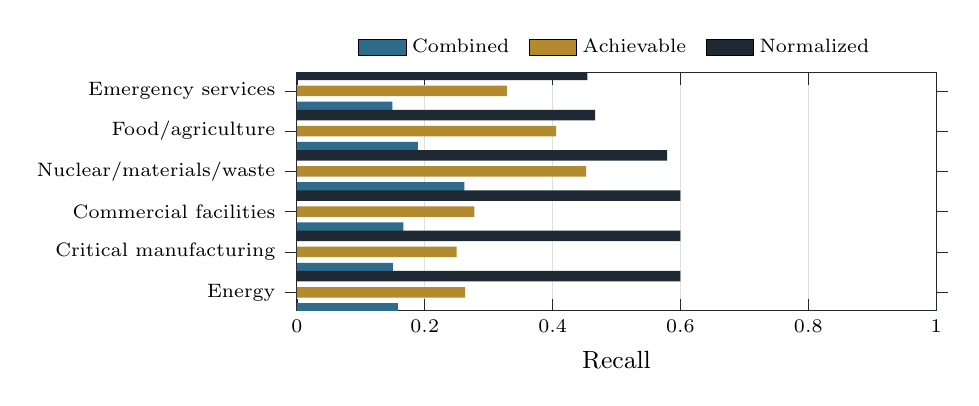
\begin{tikzpicture}
  \definecolor{pbblack}{HTML}{1F2933}
  \definecolor{pbblue}{HTML}{2F6B8A}
  \definecolor{pbgold}{HTML}{B38B2E}
  \begin{axis}[
    xbar,
    width=0.80\linewidth,
    height=4.6cm,
    xmin=0,
    xmax=1,
    xtick={0,0.2,0.4,0.6,0.8,1.0},
    xlabel={Recall},
    ytick={1,2,3,4,5,6},
    yticklabels={{Emergency services},{Food/agriculture},{Nuclear/materials/waste},{Commercial facilities},{Critical manufacturing},{Energy}},
    yticklabel style={font=\scriptsize},
    tick label style={font=\scriptsize},
    label style={font=\small},
    y dir=reverse,
    bar width=3.8pt,
    xmajorgrids,
    grid style={draw=gray!25},
    axis line style={draw=pbblack},
    tick style={draw=pbblack},
    enlarge y limits=0.09,
    legend columns=3,
    legend style={
      draw=none,
      fill=none,
      font=\scriptsize,
      at={(0.5,1.02)},
      anchor=south,
      /tikz/every even column/.append style={column sep=5pt},
    },
  ]
    \addplot[fill=pbblue,draw=none,area legend] coordinates {(0.149254,1) (0.189189,2) (0.261905,3) (0.166667,4) (0.150000,5) (0.157895,6)};
    \addlegendentry{Combined}

    \addplot[fill=pbgold,draw=none,area legend] coordinates {(0.328358,1) (0.405405,2) (0.452381,3) (0.277778,4) (0.250000,5) (0.263158,6)};
    \addlegendentry{Achievable}

    \addplot[fill=pbblack,draw=none,area legend] coordinates {(0.454545,1) (0.466667,2) (0.578947,3) (0.600000,4) (0.600000,5) (0.600000,6)};
    \addlegendentry{Normalized}
  \end{axis}
\end{tikzpicture}
